\section{步的接受与半径更新}
\label{sec:tr-acceptance}

子问题给出了一个候选步，但模型的话不能全信。这就需要回答：怎样用真实目标检验这一步，并决定下一轮用多大的半径？

\paragraph{主要思想}
第~\ref{sec:tr-model}节已经分开了预测下降和实际下降，把它们相除就是一个无量纲的检验量。定义\term{下降比}（reduction ratio）：
\begin{equation}
 \rho^{(t)}=\frac{\operatorname{ared}(\bm{p}^{(t)})}{\operatorname{pred}(\bm{p}^{(t)})}
 =\frac{f(\bm{x}^{(t)})-f(\bm{x}^{(t)}+\bm{p}^{(t)})}{m^{(t)}(\bm{0})-m^{(t)}(\bm{p}^{(t)})}.
 \label{eq:tr-rho}
\end{equation}
只要$\bm{g}^{(t)}\neq\bm{0}$且候选步满足式~\eqref{eq:tr-sufficient-decrease}，分母就为正，比值有意义。

$\rho^{(t)}$接近$1$，说明模型在这个范围内预测得准。$\rho^{(t)}$是很小的正数，说明目标虽有下降，但比预测差得多。$\rho^{(t)}$为负，说明目标实际上升了。$\rho^{(t)}$大于$1$，说明目标比模型预测的下降更多，这是好事，但也表明模型并不精确。

用两个阈值$0<\eta_1\leq\eta_2<1$把数轴分成三段，常取$\eta_1=1/4$，$\eta_2=3/4$；另取缩小因子$\theta\in(0,1)$和半径上限$\Delta_{\max}$。下一个点按是否接受决定：
\begin{equation}
 \bm{x}^{(t+1)}=
 \begin{cases}
  \bm{x}^{(t)}+\bm{p}^{(t)},&\rho^{(t)}\geq\eta_1,\\
  \bm{x}^{(t)},&\rho^{(t)}<\eta_1.
 \end{cases}
 \label{eq:tr-accept}
\end{equation}

下一轮的半径按模型的表现决定：
\begin{equation}
 \Delta^{(t+1)}=
 \begin{cases}
  \theta\Delta^{(t)},&\rho^{(t)}<\eta_1,\\
  \min\{2\Delta^{(t)},\Delta_{\max}\},&\rho^{(t)}\geq\eta_2\text{ 且步在边界},\\
  \Delta^{(t)},&\text{其他情形}.
 \end{cases}
 \label{eq:tr-radius}
\end{equation}

第二种情形多了“步在边界”这个条件，即$\lVert\bm{p}^{(t)}\rVert_2=\Delta^{(t)}$：若步在球内部，半径并没有限制住它，扩大半径没有意义。图~\ref{fig:tr-rho-decision}把这三段画在数轴上。

\begin{BookInlineFigure}
 \centering
 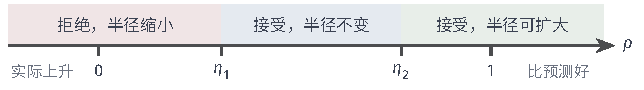
\includegraphics[width=109mm]{figures/05-optimization/02-smooth-optimization/tikz/tr-rho-decision/figure.pdf}
 \caption{下降比$\rho$的三段及相应动作。红色段拒绝这一步，蓝色段接受但半径不变，绿色段接受，并且在步到达边界时扩大半径。}
 \label{fig:tr-rho-decision}
\end{BookInlineFigure}

拒绝一步的代价比看上去小。点没有动，梯度和$\bm{B}$都不用重算，下一轮用同一个模型在更小的球里重解子问题。这里要与线搜索的回溯对比：回溯只缩短长度，方向不变；信赖域缩小半径后，新的解方向一般也变了。图~\ref{fig:tr-loop}是完整的一轮。

\begin{BookInlineFigure}
 \centering
 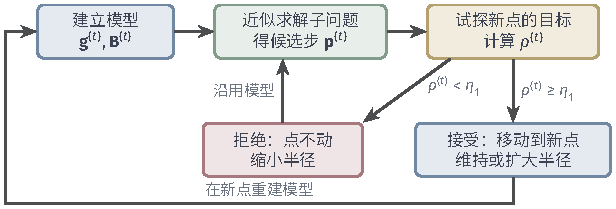
\includegraphics[width=104mm]{figures/05-optimization/02-smooth-optimization/tikz/tr-loop/figure.pdf}
 \caption{信赖域方法的一轮。黄框里的目标值是这一轮唯一一次新增的函数值计算。接受时回到左侧在新点重建模型，拒绝时模型沿用，只在更小的球内重解子问题。}
 \label{fig:tr-loop}
\end{BookInlineFigure}

\paragraph{模型矩阵从哪里来}
框架对$\bm{B}^{(t)}$的要求很少：对称，范数有界。取Hessian得到信赖域Newton法；取第~\ref{chap:quasi-newton}章的BFGS近似也可以。第~\ref{chap:quasi-newton}章的SR1更新尤其适合这里，它由位移$\bm{s}=\bm{p}^{(t)}$和梯度差$\bm{y}$得到
\begin{equation}
 \bm{B}^{(t+1)}=\bm{B}^{(t)}+\frac{(\bm{y}-\bm{B}^{(t)}\bm{s})(\bm{y}-\bm{B}^{(t)}\bm{s})^\top}{\langle\bm{y}-\bm{B}^{(t)}\bm{s},\bm{s}\rangle}.
 \label{eq:tr-sr1}
\end{equation}

SR1不保持正定性，$\bm{B}^{(t+1)}$可能不定，放进线搜索框架时方向可能不是下降方向，这在信赖域中不成问题。分母过小时跳过更新。即使这一步被拒绝，$\bm{s}$和$\bm{y}$仍然是真实的曲率信息，通常也用来更新，代价是在试探点多算一次梯度。这时$\bm{B}^{(t)}$已不是$\bm{H}^{(t)}$，下面的手算例子仍用Hessian。

\needspace{6\baselineskip}
\paragraph{变量}
下面用目标~\eqref{eq:tr-example}走完整个过程，子问题用截断共轭梯度求解。要维护的量是：
\begin{itemize}
 \item $\bm{x}^{(t)}\in\mathbb{R}^n$：当前点，$f(\bm{x}^{(t)})$是它的目标值；
 \item $\Delta^{(t)}>0$：当前半径；
 \item $\bm{g}^{(t)}\in\mathbb{R}^n$，$\bm{B}^{(t)}\in\mathbb{R}^{n\times n}$：当前模型，上一轮被拒绝时直接沿用。
\end{itemize}

\paragraph{初始化}
选定$\bm{x}^{(0)}$，$\Delta^{(0)}$，阈值和缩小因子。例中取
\[
 \bm{x}^{(0)}=\begin{bmatrix}0\\0\end{bmatrix},\qquad\Delta^{(0)}=2,\qquad\Delta_{\max}=8,
\]
\[
 \eta_1=\frac14,\qquad\eta_2=\frac34,\qquad\theta=\frac12.
\]

\paragraph{每轮更新}
第$t$轮依次执行以下步骤，直到$\lVert\bm{g}^{(t)}\rVert_2$小于给定的容差。

\begin{enumerate}
 \item 若上一轮接受了步，由式~\eqref{eq:tr-example-derivatives}计算$\bm{g}^{(t)}$和$\bm{B}^{(t)}$。例中第$0$轮得到数据~\eqref{eq:tr-data-o}。
 \item 近似求解子问题~\eqref{eq:tr-subproblem}，得到$\bm{p}^{(t)}$。例中第$0$轮就是上一节算过的曲率停止：
 \[
  \bm{p}^{(0)}=\begin{bmatrix}-1.6\\-1.2\end{bmatrix},\qquad\operatorname{pred}(\bm{p}^{(0)})=1.92.
 \]
 \item 由式~\eqref{eq:tr-rho}计算$\rho^{(t)}$。例中第$0$轮由式~\eqref{eq:tr-example-error}，模型误差是$\tfrac14(1.6)^4=1.6384$，于是
 \[
  \operatorname{ared}(\bm{p}^{(0)})=1.92-1.6384=0.2816,\qquad\rho^{(0)}\approx0.147.
 \]
 \item 由式~\eqref{eq:tr-accept}和式~\eqref{eq:tr-radius}决定下一个点和半径。例中第$0$轮$\rho^{(0)}<1/4$，拒绝这一步，并有
 \[
  \bm{x}^{(1)}=\begin{bmatrix}0\\0\end{bmatrix},\qquad\Delta^{(1)}=1.
 \]
\end{enumerate}

第$1$轮沿用同一个模型。半径变成$1$，共轭梯度的第一步$(-1,-1)^\top$长度为$\sqrt2$，已越过边界，所以截断在球面上：
\[
 \bm{p}^{(1)}=\begin{bmatrix}-1/\sqrt2\\-1/\sqrt2\end{bmatrix},\qquad\operatorname{pred}(\bm{p}^{(1)})=\sqrt2-\frac12\approx0.9142.
\]

模型误差是$\tfrac14(1/\sqrt2)^4=0.0625$，于是实际下降约为$0.8517$，比值$\rho^{(1)}\approx0.932\geq3/4$。这一步在边界上，接受并把半径扩大：
\[
 \bm{x}^{(2)}\approx\begin{bmatrix}-0.7071\\-0.7071\end{bmatrix},\qquad\Delta^{(2)}=2.
\]
半径减半之后，步的方向由$(-1.6,-1.2)$变成了负梯度方向，这正是前面说的方向随半径变化。图~\ref{fig:tr-rejection}把这两次试探画在真实目标上。

\begin{BookInlineFigure}
 \centering
 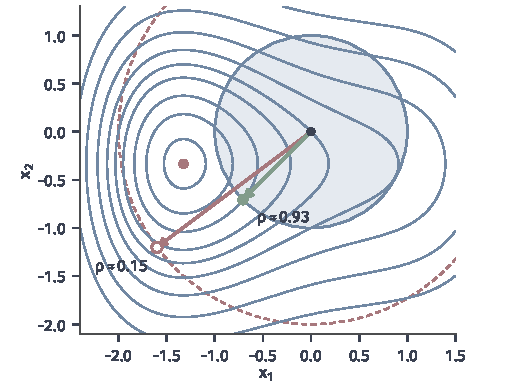
\includegraphics[width=90mm]{figures/05-optimization/02-smooth-optimization/matplotlib/tr-rejection/figure.pdf}
 \caption{原点处的一次拒绝与一次接受，蓝线是目标~\eqref{eq:tr-example}的等高线。红色虚线圆和红色箭头是$\Delta=2$的试探，空心点被拒绝；浅蓝圆盘和绿色箭头是$\Delta=1$的试探，绿点被接受。红色实心点是最小点。}
 \label{fig:tr-rejection}
\end{BookInlineFigure}

第$2$轮由式~\eqref{eq:tr-example-derivatives}重建模型：
\[
 \bm{g}^{(2)}\approx\begin{bmatrix}1.3536\\-1.1213\end{bmatrix},\qquad\bm{B}^{(2)}\approx\begin{bmatrix}0.5&0\\0&3\end{bmatrix}.
\]

这时$\bm{B}$已经正定，但$x_1$方向的曲率只有$0.5$，比前方实际的曲率小得多。$\Delta=2$的步是$\bm{p}^{(2)}\approx(-1.928,0.530)^\top$，预测下降$1.853$，实际却上升$6.674$，$\rho^{(2)}\approx-3.60$，又被拒绝。第$3$轮半径减半后，比值回到$0.589$，接受，半径保持为$1$。

继续下去，第$4$轮开始Newton步已落在球内，由残差停止，半径不再起作用，比值接近$1$，梯度范数迅速下降。表~\ref{tab:tr-history}列出全部$8$轮，最终得到$\bm{x}\approx(-1.3247,-0.3333)^\top$，$f\approx-1.5989$，这就是$\bm{x}^\star$。图~\ref{fig:tr-outer-path}是轨迹和半径的变化。

\begin{BookInlineTable}
 \centering
 \begin{tabular}{rrrcrrrl}
  \toprule
  $t$ & $f(\bm{x}^{(t)})$ & $\Delta^{(t)}$ & 停止 & pred & ared & $\rho^{(t)}$ & 结果\\
  \midrule
  $0$ & $0.000$ & $2$ & 曲率 & $1.920$ & $0.282$ & $0.147$ & 拒绝\\
  $1$ & $0.000$ & $1$ & 边界 & $0.914$ & $0.852$ & $0.932$ & 接受，扩大\\
  $2$ & $-0.852$ & $2$ & 边界 & $1.853$ & $-6.674$ & $-3.602$ & 拒绝\\
  $3$ & $-0.852$ & $1$ & 边界 & $0.999$ & $0.588$ & $0.589$ & 接受\\
  $4$ & $-1.440$ & $1$ & 残差 & $0.155$ & $0.158$ & $1.023$ & 接受\\
  $5$ & $-1.598$ & $1$ & 残差 & $0.001$ & $0.001$ & $1.011$ & 接受\\
  $6$ & $-1.599$ & $1$ & 残差 & $0.000$ & $0.000$ & $1.000$ & 接受\\
  $7$ & $-1.599$ & $1$ & 残差 & $0.000$ & $0.000$ & $0.999$ & 接受\\
  \bottomrule
 \end{tabular}
 \caption{贯穿例子的完整运行。pred和ared是预测下降与实际下降，“停止”是内层截断共轭梯度的停止原因。}
 \label{tab:tr-history}
\end{BookInlineTable}

\begin{BookInlineFigure}
 \centering
 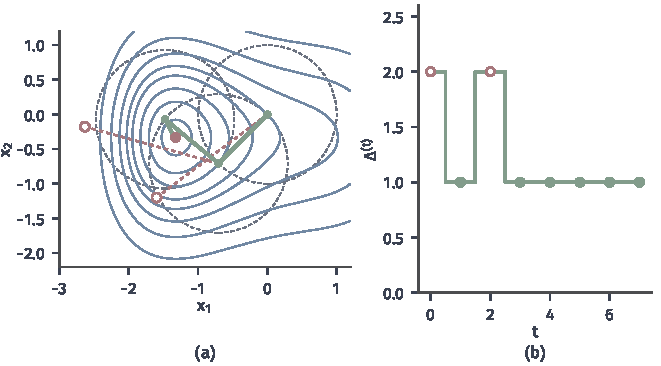
\includegraphics[width=112mm]{figures/05-optimization/02-smooth-optimization/matplotlib/tr-outer-path/figure.pdf}
 \caption{贯穿例子的完整运行。(a)~目标等高线（蓝）上的轨迹（绿），虚线圆是前几轮被接受时的信赖域，红色虚线和空心点是被拒绝的试探，红点是最小点。(b)~半径随轮数的变化，实心点表示接受，空心点表示拒绝。}
 \label{fig:tr-outer-path}
\end{BookInlineFigure}

这次运行显示了框架的分工：远离解时，半径起主导作用，负责把模型限制在可信的范围；靠近解时，半径不再起作用，方法退化成普通的Newton法。半径的调整不需要人工干预，由下降比自动完成。
